\chapter{Implementation}
\label{cha:implementation}
\section{Overview}
\label{sec:impl-overview}
The system  contains multiple microservices realized in a docker network:
\begin{itemize}
    \item \texttt{bootstrap} runs an IPFS daemon and is responsible for initializing the IPFS network, all other participants in the network connect through this node. 
    The Go implementation of \acs{IPFS} (go-ipfs\footnote{\url{https://github.com/ipfs/go-ipfs}}) is used as back-end instead the JavaScript implementation, due to performance. This is due to the goal being performance measurings, where go should perform better. The go-ipfs must run as a daemon in the background. This is tolerable, due to the vision of having IPFS implemented and running natively in the browser.
    \item \texttt{client} represents the users of the system, and there can be arbitrarily many of them depending on the test. The clients run an IPFS daemon and a browser that is controlled through Splinter, they then play various videos hosted in the network through the IPFS \acs{API} from the \texttt{dash.js} video player with different viewing patterns and connection conditions.
    \item \texttt{host} hosts the HTML website that the DASH.js player resides on, each client could host this themselves, but having it a single place makes the system more mutable.
    \item \texttt{metric} is a client to the Mongo database that is contacted by the client, the clients reguarly report data regarding their viewing session to Metric which then forwards this to the database, this data includes latency for getting a segment, whether the video halted and more.
    \item \texttt{mongo} is a dockerized Mongo database.
    \item \texttt{plot} is a Mongo client that processes the data stored in the Mongo database and presents it with various plots, it can also export this to a csv format.
    \item \texttt{pumba} is a chaos engineering tool that is used to manipulate the \texttt{client} instances in terms of their download and upload speed, latency and even shutting them down.
\end{itemize}
Relation between these services is also  illustrated in figure \ref{fig:uml_docker-compose}.

\begin{figure}[bth]
       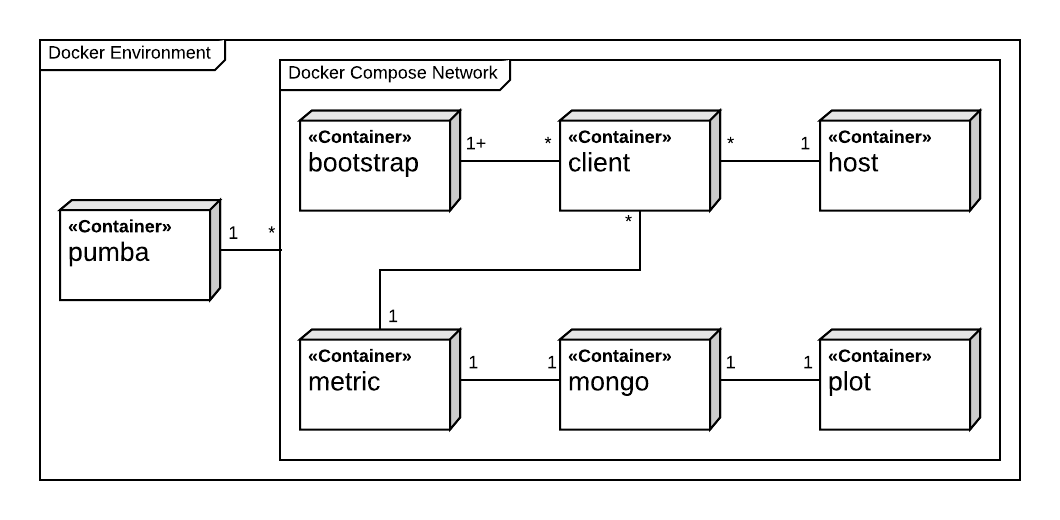
\includegraphics[width=\linewidth]{gfx/uml_docker_setup.png}
       \caption[Diagram of the experimental test  setup]{Diagram of the experimental test setup, illustrating the relations between the Docker containers described in section \ref{sec:impl-overview}.}
        \label{fig:uml_docker-compose}
\end{figure}

\section{Video Tools}

\subsection{FFmpeg}
The commandline program \texttt{ffmpeg}\footnote{\url{https://ffmpeg.org}} was used for transcoding videos to the proper codecs. The used codecs is chossen to H.264 for video and AAC for audio. 
\texttt{ffmpeg} also makes it possible to change the number of I-frames, which could be necessary due to the segmentation of the streams into multiple files in the DASHing process.

\subsection{MP4Box multimedia packager}
The tool MP4Box from the GPAC framework\footnote{\url{https://github.com/gpac/gpac}} was used to split the streams into segment files and generate a \acs{MPD}.

\section{User Emulation Tools}
\subsection{Splinter}
Splinter\footnote{\url{https://github.com/cobrateam/splinter}} is a Python library used for emulating user input through a browser. Various personas will be interacting with the website through a chrome browser by utilizing this library, and thereby emulating different types of user behaviour.

%%% Local Variables:
%%% mode: latex
%%% TeX-master: "../ClassicThesis"
%%% End:
